\documentclass[aspectratio=169]{beamer}


\usepackage[brazil]{babel}
\usepackage[utf8]{inputenc}
\usepackage{algorithm, algpseudocode}
\usepackage{graphicx}
\usepackage{subfig}
\usepackage[absolute]{textpos}
\usepackage{todonotes, verbatim}
\makeatletter
\renewcommand{\ALG@beginalgorithmic}{\small}
\makeatother

\usetheme[progressbar=foot]{metropolis}

\title{Disciplina de Metodologia Científica}
\subtitle{Estado da Arte \\Sistemas de Assistência de Direção usando \textit{Hardware} Reconfigurável}
\date{\today}
\author{Rodolfo Labiapari Mansur Guimarães}

\institute{
	\textit{rodolfolabiapari@gmail.com} \\
	Departamento de Computação -- Universidade Federal de Ouro Preto \\
		35.400-000 -- Ouro Preto - MG -- Brasil 
	}



\begin{document}
	\maketitle
  
\usebackgroundtemplate{
\includegraphics[trim=0 245cm 0 0, width=0.05\textwidth]{img/ufop.jpg}}
 
 
 \section{Apresentação}
 
 \begin{frame}{Apresentação}
 	\begin{figure}[H]
 		\centering
 		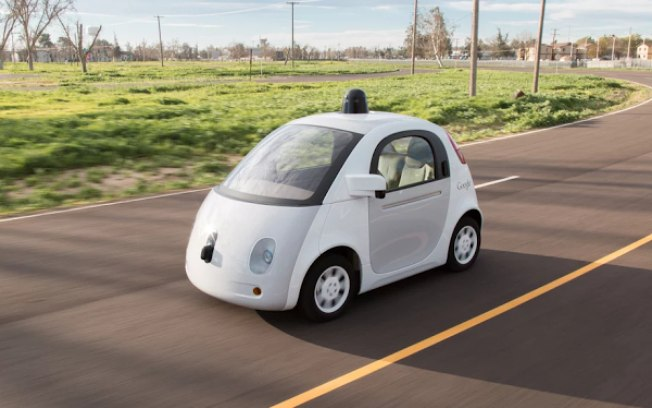
\includegraphics[width=0.78\textwidth]{img/google_car.jpg}
 		\pause
 		\caption{Carro Autônomo.}
 		\label{fig:google_car}
 	\end{figure}
 \end{frame}
 
\begin{frame}{Apresentação}
	\begin{figure}[H]
		\centering
		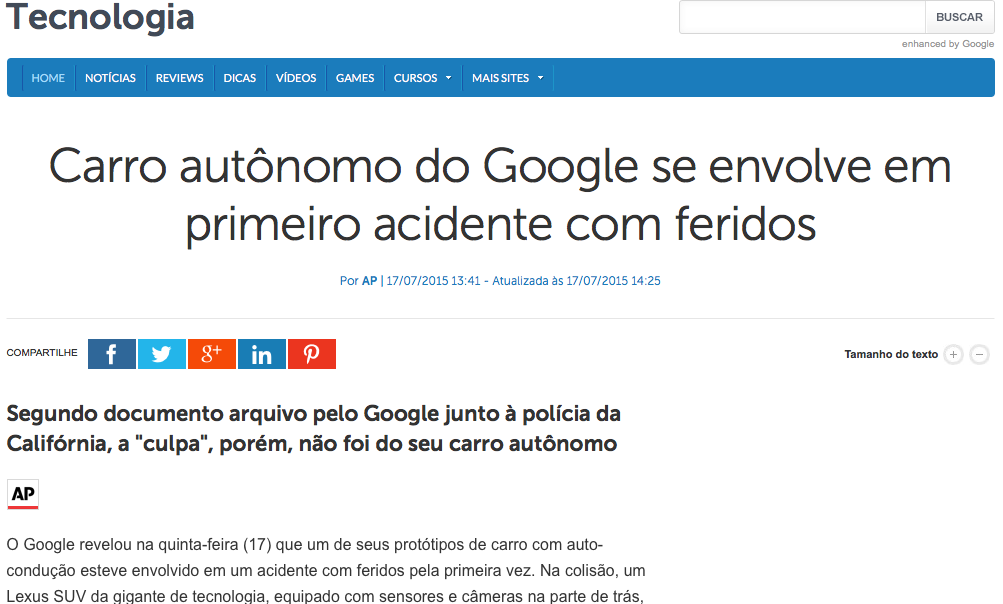
\includegraphics[width=0.75\textwidth]{img/google_car_noticia.png}
		\protect\caption{Noticiário. Fonte: \url{http://tecnologia.ig.com.br/2015-07-17/carro-autonomo-do-google-se-envolve-em-primeiro-acidente-com-feridos.html}}
		\label{fig:google_car_noticia}
	\end{figure}
\end{frame}
 


\section{Introdução ao Problema}
 
\begin{frame}{Introdução ao Problema}
	\begin{itemize}
		\item A \textbf{detecção de erros} do condutor ao dirigir é uma das questões-chaves de \textbf{Veículos Inteligentes} e de \textbf{Sistemas Avançado de Assistência de Direção (ADAS)} utilizados no tráfego.
		
		\item Atualmente, existem vários sistemas que realizam este tipo de assistência ao motorista auxiliando numa \textbf{viagem segura}.
		
		\item Utilizam meios de \textbf{percepção de discrepâncias} na condução do veículo com o propósito de:
		\begin{itemize}
			\item Organizar o trânsito; e
			\item Reduzir os acidentes.
		\end{itemize}
		
			\bigskip
		
		\item Como isso é feito? \pause Analisando \textbf{sonolência} ou \textbf{falta de atenção do motorista}.
		
		 \item Isso é possível com a ajuda de \textbf{sensores} como:
		 \begin{itemize}
		 	\item Câmeras;
		 	\item Potenciômetros; e 
		 	\item Acelerômetros.
		 \end{itemize}
	\end{itemize}
\end{frame}


\section{Características do Problema}

\begin{frame}{Características do Problema}
	\begin{itemize}
		\item Um veículo com um ADAS é comumente conhecido na literatura como um \textbf{\textit{veículo inteligente}}.
		\item Com a detecção de sinais de falta de atenção na condução de um veículo:
		\begin{itemize}
			\item Alertas podem ser emitidos a ponto de conscientizar o condutor a parar o veículo ou mesmo na intervenção direta da condução prezando pela segurança.
		\end{itemize}
		
			\bigskip
		
		 \item São \textbf{sistemas de tempo real} e devem atender exigências como:
		 \begin{itemize}
		 	\item Desempenho;
		 	\item Confiabilidade (baixa taxa de falsos positivos);  e 
		 	\item Segurança (alta taxa de precisão).
		 \end{itemize}
	\end{itemize}
\end{frame}



\section{Tecnologia Utilizada Hoje}

\begin{frame}{Tecnologia Utilizada Hoje}
	\begin{itemize}
		\item Atualmente estes sistema são fabricados utilizando circuitos integrados ASICs (\textit{Application Specific Integrated Circuit}):
		
			\bigskip
			
		\begin{itemize}
			\item Tal como são fabricados os circuitos de rádio, televisão, computador, ... \pause
			
				\bigskip
			
			\item Ou seja, \textbf{não podem ser alterados depois da fabricação}.
		\end{itemize}
	\end{itemize}
\end{frame}


\begin{frame}{Tecnologia Utilizada Hoje}
	\begin{figure}[H]
		\centering
		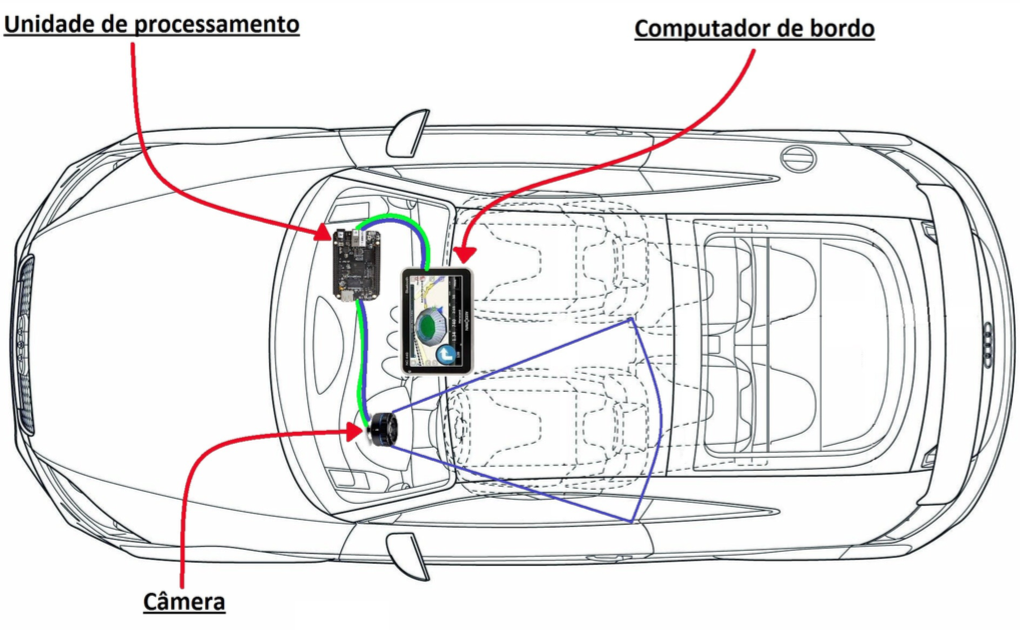
\includegraphics[width=0.75\textwidth]{img/camera_motorista.png}
		\caption{Sistema de \textit{hardware} de um Veículo Inteligente. Fonte: \cite{kitt}}
		\label{fig:sistema}
	\end{figure}
\end{frame}



\section{Tecnologia Proposta para Pesquisa}

\begin{frame}{Tecnologia Proposta para Pesquisa}
	\begin{itemize}
		\item O \textit{hardware} reconfigurável FPGA\footnote{\textit{Field Programmable Gate Array}.} é um circuito integrado que contém um grande número de \textbf{unidades lógicas idênticas} que podem ser configuradas independentemente e \textbf{interconectadas} a partir de uma matriz de trilhas condutoras e \textit{switches} programáveis.
		
		\item Diferentemente de circuitos integrados ASIC, as funções do FPGA são definidas por um programa assistido pelo computador e são facilmente modificadas:
		
		\begin{itemize}
			\item Esta flexibilidade possibilita acesso à projetos de circuitos integrados combinacionais complexos sem os altos custos de engenharia associados aos ASICs;
			\item E a programação pode ser feita com linguagem de descrição de \textit{hardware} como Verilog e VHDL\footnote{\textit{VHSIC Hardware Description Language}.}.
		\end{itemize}
	\end{itemize}
\end{frame}



\begin{frame}{Tecnologia Proposta para Pesquisa - Visão Geral}
	\begin{figure}[H]
		\centering
		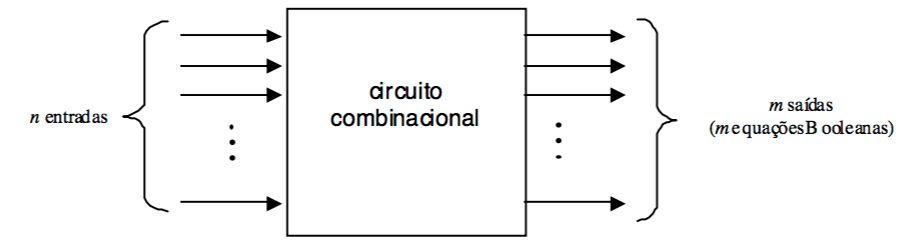
\includegraphics[width=1\textwidth]{img/geral1.png}
		\caption{Exemplo de um circuito combinacional.}
	\end{figure}
\end{frame}

\begin{comment}

\begin{frame}{Tecnologia Proposta para Pesquisa - Visão Geral}
\begin{figure}[H]
\centering
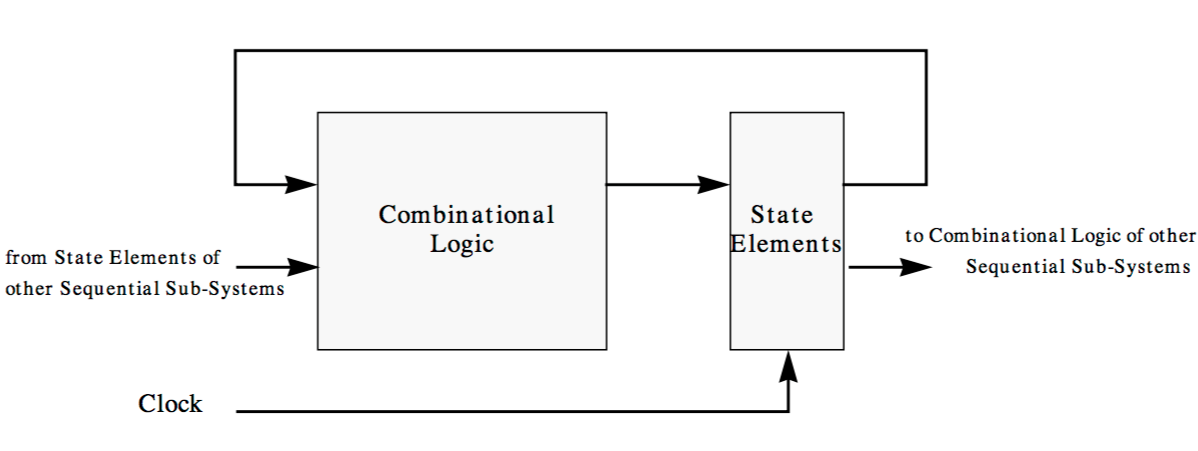
\includegraphics[width=1\textwidth]{img/geral2.png}
\caption{Exemplo de um circuito combinacional com mais detalhes.}
\end{figure}
\end{frame}
\end{comment}

\begin{frame}{Tecnologia Proposta para Pesquisa - Visão Geral}
	\begin{figure}[H]
		\centering
		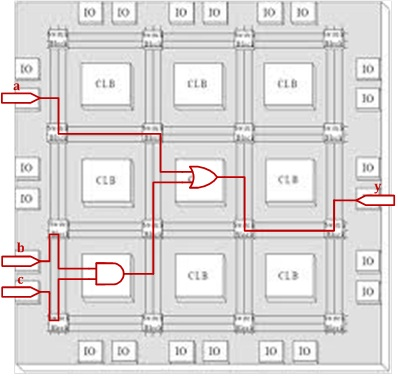
\includegraphics[width=0.5\textwidth]{img/demonstracao.jpg}
		\caption{Demonstração de síntese.}
	\end{figure}
\end{frame}

\begin{frame}{Tecnologia Proposta para Pesquisa - Visão Geral}
	\begin{figure}[H]
		\centering
		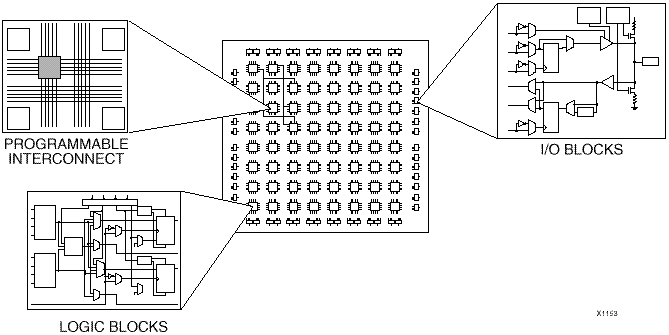
\includegraphics[width=0.97\textwidth]{img/demonstracao_2.png}
		\caption{Demonstração mais complexa de síntese.}
	\end{figure}
\end{frame}

\begin{frame}
	\begin{figure}[H]
		\centering
		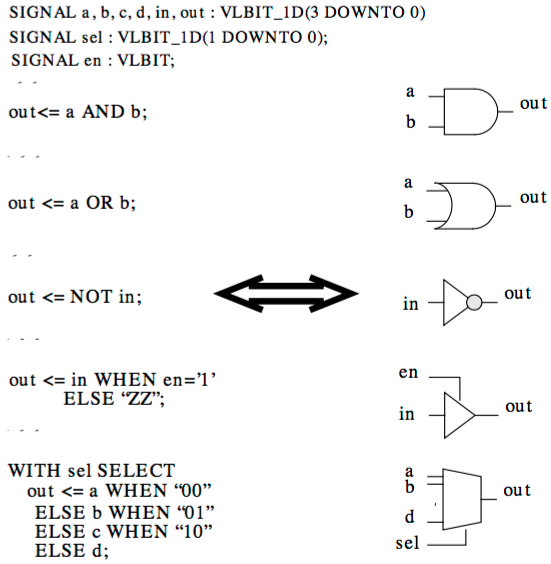
\includegraphics[width=0.6\textwidth]{img/linguagem.png}
		\caption{Exemplo de linguagem de descrição de \textit{hardware} utilizada para projeção e síntese.}
	\end{figure}
\end{frame}

\begin{frame}
	\begin{figure}[H]
		\centering
		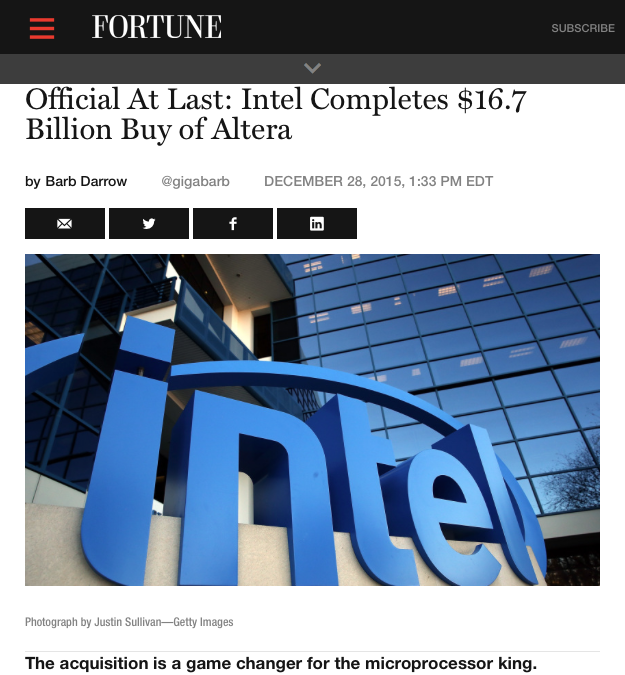
\includegraphics[width=0.5\textwidth]{img/intel_altera_2.png}
		\protect\caption{Noticiário. Fonte: \url{http://fortune.com/2015/12/28/intel-completes-altera-acquisition/}}
		\label{fig:intel_altera_noticia}
	\end{figure}
\end{frame}


\section{Estado da Arte}
\begin{frame}{Estado da Arte - Principais Meios de Publicação}
	\begin{itemize}
		\item Verificou-se sobre o tema utilizando as palavras-chaves relativas às respectivas grandes áreas: 
		\begin{itemize}
			\item \textbf{\textit{ADAS} e \textit{Vehicular-Intelligent}}: para veículos inteligentes; e \item \textbf{\textit{FPGA} e \textit{Hardware-Reconfigurable}} para dispositivos reconfiguráveis.
		\end{itemize} 
		
			\bigskip
		
		\item Foram realizadas pesquisas nos principais meios de publicações existentes sendo alguns deles os \textit{journals} e conferências:
	\end{itemize}
\end{frame}


\begin{frame}{Estado da Arte - Principais Journals e Conferências das Áreas}
	
	{\it \scriptsize 
		\begin{itemize}
         \item \textbf{A2} ACM/SIGDA International Symposium on Field-Programmable Gate Arrays;
         \item \textbf{A2} International Conference on Field Programmable Logic and Applications;
         \item \textbf{B3} ACM Transactions on Reconfigurable Technology and Systems;
         \item \textbf{B3} International Conference on Engineering of Reconfigurable Systems and Algorithms (ERSA);
         \item \textbf{B3} Reconfigurable Architectures Workshop (RAW);
         \item \textbf{B4} International Conference on Reconfigurable Computing and FPGAs (ReConFig);
         \item \textbf{B4} International Journal of Reconfigurable Computing (Print)
         \item \textbf{B4} International Workshop on Reconfigurable Communication-centric Systems-on-Chip (ReCoSoC);
         \item \textbf{--} International Workshop on Applied Renconfigurable Computing (ARC);
         \item \textbf{--} International Workshop on Distributed Auto-Adaptive and Reconfigurable Systems (DARES@ICDCS);
         \item \textbf{--} International Workshop on High-Performance Renconfigurable Computing Technology and Applications (HPRTCA@SC);
         \item \textbf{--} International IEEE Symposium on Field-Programmable Custom Computing Machines;
         \item \textbf{--} International Conference on Field-Programmable Technology;
		\end{itemize}
	}
\end{frame}


\begin{frame}{Estado da Arte - Primeiras Impressões}
	\begin{itemize}
		\item A priori, não existe nenhum tipo de \textbf{meio de publicação} que aborde as duas áreas \textbf{simultaneamente}:
		
		\item Por isso, analisou-se cada uma dos meios a procura de artigos que abordem as duas matérias.
	\end{itemize}
\end{frame}

\begin{frame}{Estado da Arte}
	\begin{itemize}
		\item Por exemplo, o trabalho de Kumar \cite{seis} que possui:
		\begin{itemize}
			\item Um detector de sonolência;
			\item Detecção de faixas, pedestres e carros que estão a uma distância insegura;
			\item Além de sinais sonoros.
		\end{itemize} 
		
			\bigskip
		
		\item Wang \cite{sete} propôs um sistema com auto-aprendizagem que inclui:
		\begin{itemize}
			\item Controle de velocidade; e 
			\item Aviso de colisão frontal.
		\end{itemize} 
		
			\bigskip
		
		\item Chien \cite{oito} propôs um sistema que utiliza:
		\begin{itemize}
			\item  Câmera para analisar o condutor e detecção de obstruções e pedestres no caminho;
			\item Detecta faixas da pista, veículos, e pedestres.
		\end{itemize}
		
		\bigskip
		\pause
		\item \textbf{Entretanto, nenhum utilizando um FPGA}. 
		
	\end{itemize}
\end{frame}
		
\begin{frame}{Estado da Arte}
	\begin{itemize}
		\item Nas publicações de \textit{hardware} reconfigurável, Kiokes \cite{kiokes2011design} propõem um sistema avançado de serviços e comunicação veicular. 
		\begin{itemize}
			\item Consiste no design e implementação de um sistema de multiplexação ortogonal por divisão de frequência (OFDM) customizado para rede \textit{ad-hoc} veicular;
			\item Baseia-se no IEEE 802.11p, padrão de comunicação para ambientes veiculares publicado em 2010;
			\item Ou seja, trabalha-se sobre no tema de comunicação e não de assistência/segurança.
		\end{itemize}
	\end{itemize}
\end{frame}


\begin{frame}{Estado da Arte - UFOP}
	\begin{itemize}
		\item Atualmente, o Laboratório iMobilis possui alguns projetos que relacionam com esta área de pesquisa. 
		
		\begin{figure}[H]
			\centering
			\includegraphics[width=0.3\textwidth]{img/imobilis.png}
			\caption{Laboratório iMobilis.}
			\label{fig:ufop}
		\end{figure}
		
			\bigskip
		
		\item Seu sistema possui câmeras voltadas para a estrada e motorista, além de sensores no pedal de freio e volante \cite{kitt}. 
		
			\bigskip
		
		\item Entretanto, mesmo com a existência deste projeto e \textbf{possuir os equipamentos}, o laboratório não realiza pesquisa nesta área.
		
	\end{itemize}
\end{frame}


\begin{frame}{Estado da Arte na UFOP}
	\begin{figure}[H]
		\centering
		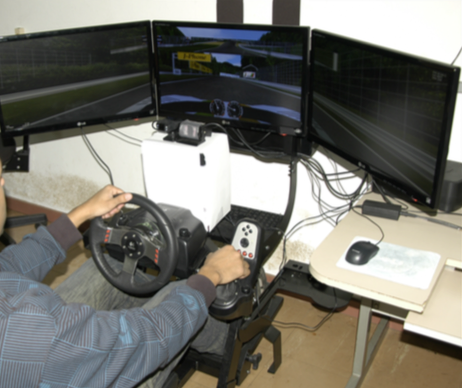
\includegraphics[width=0.55\textwidth]{img/foto1.png}
		\caption{Projeto de ADAS da UFOP num local virtual. Fonte: \cite{kitt}.}
		\label{fig:naoponderado}
	\end{figure}
\end{frame}

\section{Proposta de Pesquisa}
\begin{frame}{Proposta de Pesquisa}
	\begin{itemize}
		\item A proposta aqui apresentada é o \textbf{desenvolvimento de um ADAS numa plataforma reconfigurável} para análise de desempenho com ou outros sistemas desenvolvidos.
	\end{itemize}
\end{frame}

\maketitle

\section{Bibliografia}

\bibliographystyle{abbrv}
\bibliography{sbc-template}

\maketitle
\end{document}
